% !TEX root = ../../thesis.tex
%______________________________________________________________________________
%
% SECTION
\section{The Finite Cell Method}
\label{section:fcm}
%
%______________________________________________________________________________

Generating a boundary-conforming mesh can be costly or in some cases impossible,
especially when the model has a complex geometry, must be manipulated procedurally throughout the lifetime
of the analysis, or is represented by a geometric model that is not suitable for standard mesh generation, like point clouds.
Such is the case with inverse analyses and optimal control problems, where either
a set of boundary conditions, or the geometry itself is updated in each iteration of an
optimization process. In such cases, generating and tweaking a mesh by hand is infeasible not only because the vast amount of time it would require, but also because the quality of the mesh has a great impact on the results' accuracy and may prohibit the optimization from converging. A number of approaches exist that aim to simplify or avoid the issues of mesh generation such as Generalized Finite Element Methods (GFEM) \cite{Babuska2004} or meshless methods \cite{Chen2006}. Fictitious domain methods address the problem by extending the domain of computation such that it can be easily meshed, and introduce non-uniform material properties that separate the physical and fictitious domains. This approach shifts the focus from the meshing process to numerical integration, which is not
without its own challenges, but is more suited for automation.

The Finite Cell Method (FCM) is a fictitious domain method that works with a non-boundary-conforming
simple (often Cartesian) mesh over an embedding domain  $\Omega$, and introduces an indicator function $\alpha(\mathbf x)$ that defines the
physical domain $\Omega_p \subset \Omega$ (also called the embedded domain) in space. 

\begin{figure}[h] \label{fig:fcm_potato}
	\centering
	\begin{subfigure}[t]{0.49\textwidth}
		\centering
		\raisebox{-\height}{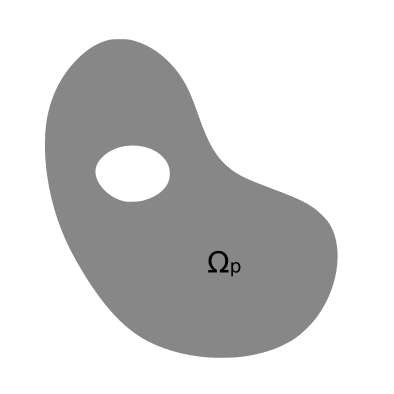
\includegraphics[height=5cm]{figures/fcm_potato.png}}
		\caption{Physical domain}
	\end{subfigure}
	%\hfill
	\begin{subfigure}[t]{0.49\textwidth}
		\centering
		\raisebox{-\height}{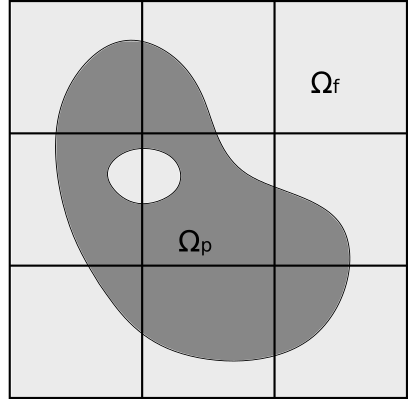
\includegraphics[height=5cm]{figures/fcm_potato_meshed.png}}
		\caption{Meshed embedding domain}
	\end{subfigure}
\caption{Example of an FCM mesh embedding the physical domain}
\end{figure}

\begin{equation} \label{eq:indicator_function}
	\alpha (\mathbf x) = \left\{
	\begin{array}{ll}
		1 & \mathbf x \in \Omega_p \\
		10^{-\beta} & \mathbf x \in \Omega_f \\
	\end{array}
	\right.
\end{equation}

The indicator function $\alpha(\mathbf x)$ is used as a coefficient for material properties, effectively "softening" the material in the fictitious domain such that the influence of its solution field on that of the physical domain becomes negligible.
Ideally, $\beta \to \infty$ leading to $\alpha (\mathbf x) \to 0$ in the fictitious domain, but is usually limited to $\beta \in [3,10]$ in order to avoid ill-conditioned structural matrices \cite{Parvizian2007}.

\begin{equation} \label{eq:fictitious_material_properties}
	\begin{array}{ll}
	\tilde \rho (\mathbf x) &= \alpha (\mathbf x) \rho \\
	\tilde E(\mathbf x) &= \alpha (\mathbf x) E
	\end{array}
\end{equation}

This modification creates discontinuous material properties in
elements that are intersected by the boundary of the physical domain (cut cells), which
in turn makes standard gaussian quadrature infeasible for the integration
of structural components (mass matrix, stiffness matrix, etc.). Methods that address this issue are presented later in this section.

The FCM primarily uses p- and hp-refinement, requiring an appropriate family of basis functions. The most common choice are integrated Legendre polynomials \cite{Duester2007} not only because of their hierarchical properties, but the $d$ dimensional tensor product space constructed from them can be truncated while preserving its completeness. This greatly reduces the number of degrees of freedom at higher polynomial orders, especially in 3D.

Considering that the shape of the physical domain must be captured during integration, and the high polynomial order of the ansatz space, an appropriate choice of integration scheme for cut cells is key to obtaining accurate results. Several methods exist
to capture discontinuities in numerical integration but two adaptive schemes are covered here in detail,
both of which rely on cartesian space partitioning trees: a standard quadtree/octree partitioned
quadrature and moment fitting.

%______________________________________________________________________________
% SUB-SECTION
\subsection*{Numerical Quadrature}
\label{subsection:numerical_quadrature}
%______________________________________________________________________________

Each considered integration scheme is based on numerical quadrature, that approximates an integral with a weighted sum of samples of the integrand at specific locations \cite{Atkinson1988}.

\begin{equation}
	\int_{\Xi} g(\boldsymbol{\xi}) d\boldsymbol{\xi} \approx \sum_{k=1}^m g(\boldsymbol{\xi}_k) w_k
\end{equation}

where the integrand $g(\boldsymbol{\xi})$ is evaluated over a normalized integration domain $\Xi = [-1,1]^n$ of $n$ dimensions at $m$ sample points $\boldsymbol{\xi}_k$, each multiplied with its corresponding weight $w_k$. Integrating over a different domain can be carried out after a change of variables.

For fundamental quadrature schemes such as the Gauss-Legendre or Gauss-Lobatto rules, the number of sample points $m$ defines the order of integration. These methods are typically most suited for polynomial or smooth integrands, that can be well approximated by polynomials. Each scheme is capable of exactly integrating polynomials up to a maximum order $p_m$ which scales linearly with the integration order $m$.

The preferred method of computing the structural components of uncut cells in the FCM is the Gauss-Legendre quadrature, as it offers the highest maximum order $p_m^{Leg}$ of all fundamental quadrature rules.

\begin{equation} \label{eq:gauss_legendre_maximum_order}
	p_m^{Leg} = 2m - 1
\end{equation}

%______________________________________________________________________________
% SUB-SECTION
\subsection*{Adaptive Quadrature}
\label{subsection:adaptive_quadrature}
%______________________________________________________________________________

Since the modified material properties break the smoothness of the integrands in \ref{eq:structural_components} for cut cells, standard quadrature rules can not be efficiently applied. A simple solution is to separate the domain of integration along the discontinuities and perform the quadrature on them individually, then sum up their contributions.

\begin{equation}
	\int_{\Omega} \alpha (\mathbf x) g(\mathbf x) d\mathbf x=
	\int_{\Omega_p} 1 \cdot g(\mathbf x) d\mathbf x
	+
	\int_{\Omega_f} 10^{-\beta} g(\mathbf x) d\mathbf x
\end{equation}

 The standard approach in FCM is to recursively generate subcells using a quadtree (2D) or octree (3D) and carry out the integration once a desired depth or error has been reached. Figure \ref{fig:fcm_potato_partitioned} shows a 2D example of a quadtree of depth two. Note, that this is a refinement of the integration mesh, not the finite element mesh. Hence, no additional degrees of freedom are introduced.

\begin{figure}[h]
	\centering
	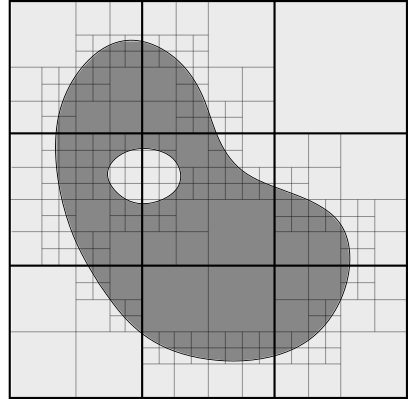
\includegraphics[height=5cm]{figures/fcm_potato_subdivided.png}
	\caption{Embedding mesh subdivided with a quadtree of depth 2.}
	\label{fig:fcm_potato_partitioned}
\end{figure}

The integration order of the underlying standard quadrature scheme is retained, and can be fully exploited if the domain boundaries are captured exactly. While this algorithm is capable of computing the desired integral up to arbitrary precision, it involves evaluating the integrands in \ref{eq:structural_components}, a series of matrix-matrix and matrix-vector multiplications, at all integration points of each subcell, thus imposing a major computational burden.

%______________________________________________________________________________
% SUB-SECTION
\subsection*{Moment Fitting}
\label{subsection:moment_fitting}
%______________________________________________________________________________

Some of the computational load introduced by adaptive integration can be reduced
with moment fitting \cite{Joulaian2015}. While the process' complexity remains exponential in terms of refinement depth, the tasks performed at each integration point can be simplified. Moment fitting is a method for generating quadrature rules on arbitrary domains \cite{Muller2013}. In the context of this thesis, it is used to preserve the number and location of integration points of the original quadrature scheme used for uncut cells, but adjust their weights by taking the integrand's discontinuities into account.

In general, a new quadrature rule defined by its nodes $\boldsymbol{\xi}_k$ (integration points) and weights $w_k$ is generated by solving the moment fitting equations

\begin{equation} \label{eq:moment_fitting}
		\sum_{k=1}^m g_j(\boldsymbol{\xi_k}) w_k = \int_{\Xi_a} g_j(\boldsymbol{\xi}) d\boldsymbol{\xi}
\end{equation}

where $g_j$ is a set of $n$ chosen basis functions. The integrals over the arbitrary domain $\Xi_a$ on the right hand side are called moments, hence the name of the method. Without any constraints, solving \ref{eq:moment_fitting} for the nodes and weights is not trivial. However, fixing the location of the integration points $\boldsymbol{\xi_k}$ transforms it into a linear system. Furthermore, choosing the basis functions $g_j$ to be Lagrange polynomials over $\boldsymbol{\xi}_k$ further simplifies the process by diagonalizing the coefficient matrix, leading to equation \ref{eq:moment_fitting_simplified}. Note that this process of simplification is identical to the premise of the Spectral Element Method in \ref{section:sem}.

\begin{equation} \label{eq:moment_fitting_simplified}
	\begin{bmatrix}
		g_1(\boldsymbol{\xi}_1) & & \\
		& \ddots & \\
		& & g_m(\boldsymbol{\xi}_m) \\
	\end{bmatrix}
	\begin{bmatrix}
		w_1 \\
		\vdots \\
		w_m \\
	\end{bmatrix}
	=
	\begin{bmatrix}
		\int_{\Xi_a} g_1(\boldsymbol{\xi}) d\boldsymbol{\xi} \\
		\vdots \\
		\int_{\Xi_a} g_m(\boldsymbol{\xi}) d\boldsymbol{\xi} \\
	\end{bmatrix}
\end{equation}

% TODO: I'm missing a source here
The integrals on the right hand side of \ref{eq:moment_fitting_simplified} can be computed with an adaptive quadrature described before, with the difference that in this case, the integrands are much cheaper to evaluate. However, the resulting quadrature rule can only integrate polynomials up to order $p_m^{MF}=m+1$ exactly, in contrast to $p_m^{Leg}=2m-1$ for the Gauss-Legendre scheme. This is due to the fact that the positions are fixed and only the weights are considered as unknowns in the moment fitting equations.
Furthermore, this assumes that the integrals on the right hand side of \ref{eq:moment_fitting_simplified} are computed exactly, which in turn implies that the geometry of the physical domain can be captured exactly by the applied space partitioning tree. This is rarely the case, but considering the fact that adaptive integration suffers from this issue as well, it is not regarded as a disadvantage of moment fitting. The reduced accuracy of the quadrature rule can be addressed by increasing the integration order of the underlying scheme.

% TODO: what's a good figure for moment fitting?

Working on a non-boundary conforming mesh introduces numerous other challenges, such as the enforcement of boundary conditions, but since a detailed literature is available on them \cite{Duester2007, Parvizian2007} and are handled identically for the SCM, they are not covered in this thesis.